
\section{Example}

The example is a simple "hello world" program, as this was practically
the only program that was able to pass through the entire pipeline. Following
is the "hello world" program written in Haskell.

\subsection{Haskell code}

\lstinputlisting[language=Haskell]{"../interpreter/tests/helloworld/helloworld.hs"}

\subsection{Converted to Core}

After the program has passed through GHC and the External-core file
has been generated, the program looks like this:

\lstinputlisting{"../interpreter/tests/helloworld/helloworld.hcr"}

\subsection{Converted to JSCore}

In the next step it is parsed and dumped to JSCore:

\lstinputlisting{"../interpreter/tests/helloworld/helloworld.hcj"}

\subsection{JSCore graph}

Using some libraries from PyPy we can generate a nice graph,
directly corresponding to the datastructure generated from parsing. 
See figure \ref{helloworldgraph}.
By simply traversing this datastructure we can generate the AST for the Core' 
interpreter (Haskell-Python).

\begin{sidewaysfigure}
\begin{figure}[H]
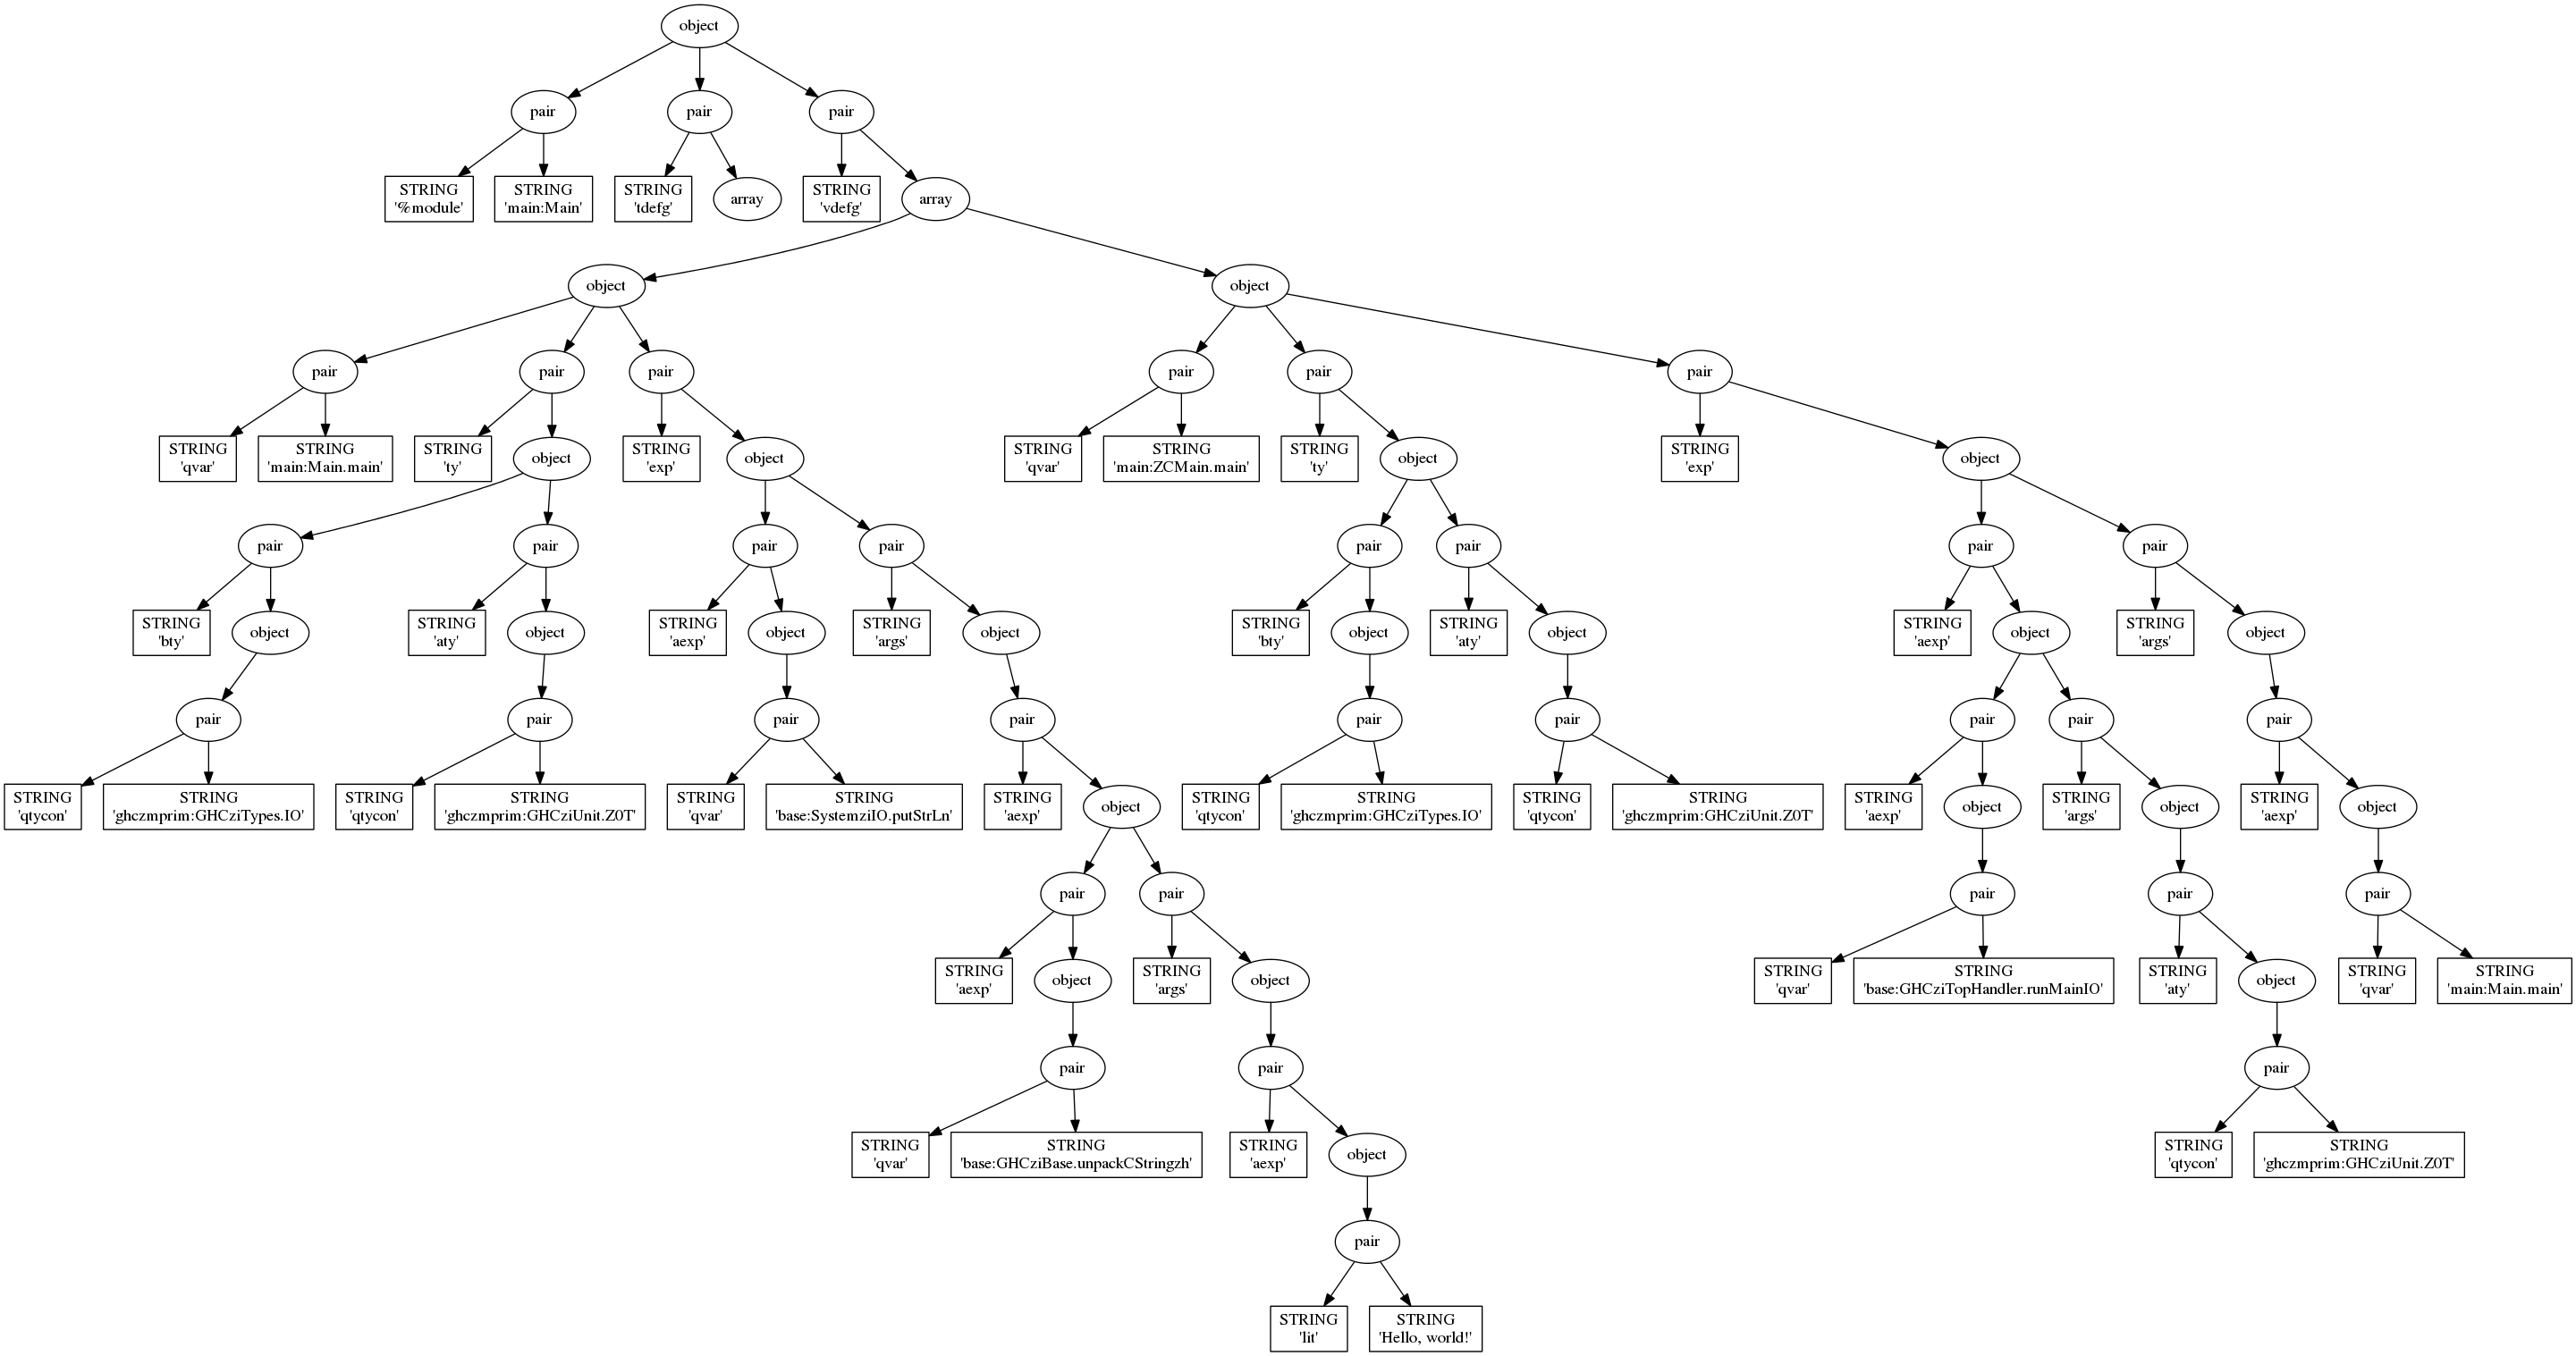
\includegraphics[width=\textwidth]{../interpreter/tests/helloworld/helloworld.png}
\caption{Example program translated to JSCore}
\label{helloworldgraph}
\end{figure}
\end{sidewaysfigure}




\subsection{Result}

The program results as expected, outputting the string "Hello, world!".









\begin{comment}

\subsection{Example 2: naive fibonacci}

The following program is a simple fibonacci program.

\lstinputlisting[language=Haskell]{"../interpreter/tests/fibonacci/fibonacci.hs"}

\subsubsection{Converted to Core}

As we can see, the simple hello world program becomes more complex when translated
to Core by GHC.

\lstinputlisting{"../interpreter/tests/fibonacci/fibonacci.hcr"}

\subsubsection{Converted to JSCore}

And translated to JSCore by our serializer:

\lstinputlisting{"../interpreter/tests/fibonacci/fibonacci.hcj"}

\subsubsection{Result}

\end{comment}
